Tras establecer los parámetros necesarios correspondientes a la gestión del proyecto, este capítulo presenta el diseño del sistema implementado. Para ello se introducirá la estructura de directorios utilizada, el diagrama del software desarrollado y la gestión de las herramientas con el protocolo MCP. 

\section{Estructura del proyecto}
El proyecto se divide en cuatro contenedores separados, cada uno con su propio entorno virtual de python venv. La figura \ref{fig:dir_principales} muestra un resumen de los directorios.

\begin{figure}[p]
\centering
\definecolor{folderbg}{RGB}{124,166,198}
\definecolor{folderborder}{RGB}{110,144,169}
\newlength\Size
\setlength\Size{4pt}
\tikzset{%
  folder/.pic={%
    \filldraw [draw=folderborder, top color=folderbg!50, bottom color=folderbg] (-1.05*\Size,0.2\Size+5pt) rectangle ++(.75*\Size,-0.2\Size-5pt);
    \filldraw [draw=folderborder, top color=folderbg!50, bottom color=folderbg] (-1.15*\Size,-\Size) rectangle (1.15*\Size,\Size);
  },
  file/.pic={%
    \filldraw [draw=folderborder, top color=folderbg!5, bottom color=folderbg!10] (-\Size,.4*\Size+5pt) coordinate (a) |- (\Size,-1.2*\Size) coordinate (b) -- ++(0,1.6*\Size) coordinate (c) -- ++(-5pt,5pt) coordinate (d) -- cycle (d) |- (c) ;
  },
}
\forestset{%
  declare autowrapped toks={pic me}{},
  declare boolean register={pic root},
  pic root=0,
  pic dir tree/.style={%
    for tree={%
      folder,
      font=\ttfamily,
      grow'=0,
      % Reducción del espaciado vertical entre nodos
      s sep=0.2cm,
      % Reducción del espaciado horizontal entre niveles
      l sep=0.8cm,
    },
    before typesetting nodes={%
      for tree={%
        edge label+/.option={pic me},
      },
      if pic root={
        tikz+={
          \pic at ([xshift=\Size].west) {folder};
        },
        align={l}
      }{},
    },
  },
  pic me set/.code n args=2{%
    \forestset{%
      #1/.style={%
        inner xsep=2\Size,
        pic me={pic {#2}},
      }
    }
  },
  pic me set={directory}{folder},
  pic me set={file}{file},
}
\begin{forest}
  pic dir tree,
  pic root,
  for tree={% folder icons by default; override using file for file icons
    directory,
  },
  [tfg\_agentes\_software
    [servidor\_mcp\_bd\_codigo
    [src
    [mcp\_code\_server.py, file]
    ]
    [...]
    ]
    [servidor\_mcp\_confluence]
    [servidor\_mcp\_google\_drive]
    [sistema\_agentes
    [src
    [db]
    [evaluators]
    [formatter\_agent]
    [orchestrator\_agent]
    [planner\_agent]
    [specialized\_agents
    [citation\_tools]
    [confluence\_agent]
    [filesystem\_agent]
    [gitlab\_agent]
    [google\_drive\_agent]
    [SpecializedAgent.py, file]
    ]
    [BaseAgent.py, file]
    [main\_graph.py, file]
    [structured\_output\_validator.py, file]
    [utils.py, file]
    ]
    [static
    [gen\_docs
    ]
    [agent\_descriptions.py, file]
    [prompts.py, file]
    ]
    [main.py, file]
    [config.py, file]
    [.env, file]
    ]
  ]
\end{forest}
\caption{Estructura de directorios principales del proyecto}
\label{fig:dir_principales}
\end{figure}

El directorio \textit{sistema\_agentes} contiene todos los agentes desarrollados junto a los clientes MCP. La implementación de los agentes se encuentra en el directorio \textit{src}, mientras que \textit{static} contiene los prompts utilizados, las descripciones de los agentes y la ``documentación oficial'' generada. El fichero \textit{.env} se encarga de almacenar variables secretas como las claves de acceso a APIs, mientras que el fichero \textit{config.py} se encarga de almacenar variables globales como el modelo por defecto utilizado en los agentes. El fichero \textit{main.py} contiene la lógica de ejecución raíz, mientras que \textit{src/main\_graph.py} contiene la implementación del agente Main.

Los directorios \textit{servidor\_mcp\_bd\_codigo}, \textit{servidor\_mcp\_confluence} y \textit{servidor\_mcp\_google\_drive} contienen cada uno un servidor MCP de ejecución independiente. 
\section{Diseño de agentes}

LangGraph proporciona un marco de trabajo estructurado para la creación de flujos de ejecución en forma de grafo. Se construye inicialmente un grafo mediante el objeto StateGraph, el cual establece la lógica de enrutamiento entre diversos nodos definidos como funciones de Python. Estos grafos utilizan un denominado estado, representado por un diccionario tipado, para almacenar el estado de ejecución durante el proceso.

Bajo este paradigma, un agente puede representarse como un grafo compilado, donde uno o varios nodos definen la lógica de invocación a los modelos LLM, mientras que otros nodos se encargan de interpretar el resultado. En una implementación tradicional, el estado conservaría los mensajes generados entre llamadas, lo que posibilita un proceso iterativo en el cual el nodo de invocación al LLM se ejecuta repetidamente, añadiendo un nuevo mensaje al estado en cada ciclo de ejecución.
\todo[inline]{Los dos párrafos anteriores quizás quedarían mejor en una breve sección en antecedentes?}

Este enfoque proporciona un marco de trabajo orientado a la composición, puesto que un nodo puede constituir a su vez otro grafo compilado que represente a otro agente. Sin embargo, presenta una problemática de redundancia: cuando dos agentes comparten gran parte del grafo que los compone, para evitar la duplicación de código sería necesario desarrollar un grafo que contemple la ejecución de ambos tipos de agentes, determinando en cada instancia cuál ejecutar en función de un parámetro presente en el estado. Aunque esta solución es viable, la programación orientada a objetos ofrece una alternativa más elegante: la herencia.

Es por este motivo que se ha optado por un enfoque híbrido que combina composición y herencia. Cada agente está implementado mediante una clase de Python, la cual contiene una función que compone el grafo representativo de la ejecución del agente. De esta manera, la clase del agente define las funciones que representan cada nodo del grafo, pudiendo heredar aquellas definidas en clases más abstractas.

Adicionalmente, esta metodología facilita el almacenamiento de datos no vinculados a la ejecución individual. Los datos encapsulados en los atributos de las clases representan información invariable en cada ejemplo de ejecución, como el nombre del agente o las herramientas disponibles; mientras que los atributos almacenados en el estado del grafo son específicos de la ejecución, como los mensajes generados durante la instancia de ejecución concreta.

\subsection{Diagrama de agentes}

\begin{figure}[p]
  \centering
  \adjustbox{center=\textwidth}{\hspace{-1cm}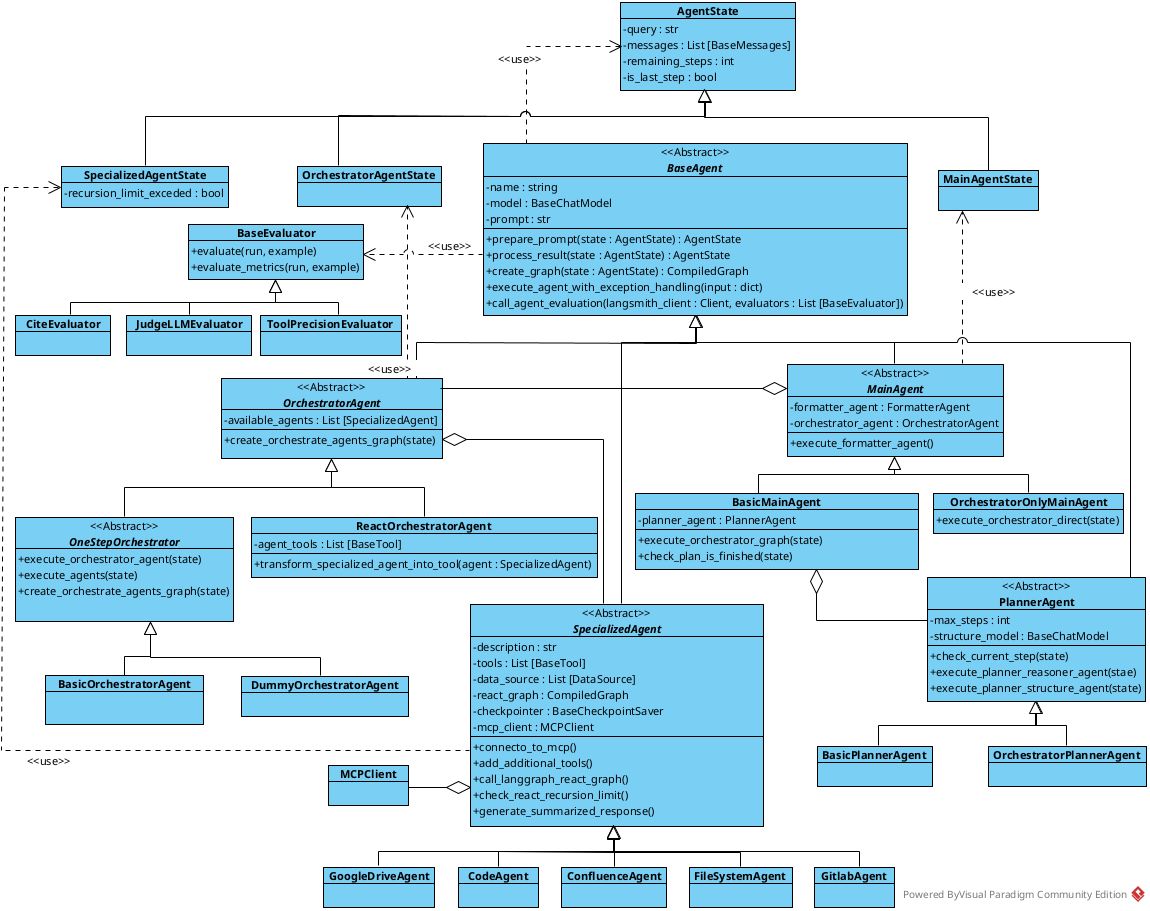
\includegraphics[width=1.35\linewidth]{figures/agentes.png}}
  \caption{Diagrama de clases UML de del sistema de agentes.}
  \label{fig:uml}
\end{figure}

La figura \ref{fig:uml} muestra el diagrama de clases (UML) general del sistema. La clase abstracta \textit{BaseAgent} define las funcionalidades básicas de todos los agentes: 
\begin{itemize}
  \item\textbf{Lógica de ejecución: }La función \textit{execute\_agent\_with\_exception\_handling} se encarga de invocar el grafo definido en \textit{create\_graph}, gestionando las excepciones e indicando los parámetros de entrada. Todos los agentes deben implementar la función \textit{prepare\_prompt}, e incluirla en su grafo de ejecución.
  \item\textbf{Gestión del resultado: }La función \textit{process\_result} se encarga de estáticamente devolver el resultado de ejeución del agente para dado un estado de ejecución. 
  \item\textbf{Evaluación del agente }La función \textit{call\_agent\_evaluation} se encarga en cada caso de definir la lógica de evaluación utilizando las métricas indicadas para cada agentes, representadas por la clase \textit{BaseEvaluator}. El capítulo \textbf{ref} explica este proceso en detalle.
\end{itemize}


Los agentes que heredan del agente base son los siguientes:
\begin{itemize}
  \item\textbf{SpecializedAgent: }Representa a los agentes que buscan en las fuentes de información especializadas, se explica en detalle en la sección \textbf{ref}. Define la lógica de gestión de las herramientas utilizadas mediante el cliente mcp, utilizando la clase Singleton \textit{MCPClient}, la cual encapsula la lógica de conexión con todos los servidores MCP disponibles, explicado en la sección \textbf{ref}. También contiene una secuencia de instancias de \textit{DataSource}, las cuales definen todos los documentos citables en las fuentes de datos disponibles, véase la sección \textbf{ref}.
  \item\textbf{OrchestratorAgent: }Implementa la lógica de enrutamiento de los agentes especialistas, decidiendo en cada caso cuáles agentes utilizar para una questión dada. Véase la sección \textbf{ref}. 
  \item\textbf{PlannerAgent: }Define la lógica de planificación a seguir para una consulta dada, creando planes secuenciales dinámicamente ajustables. Véase la sección \textbf{ref}.
  \item\textbf{FormatterAgent: }Convierte una secuencia de ejecución de agentes en un resultado legible, compuesta por una respuesta en formato textual y un conjunto de citas referenciando a documentos del proyecto software. Véase sección \textbf{ref}.
  \item\textbf{MainAgent: }Define el flujo general de la ejecución, especificando si se usarán agentes planfiicadores, orquestadores y concatenando su respueta al agente formateador. Véase la sección \textbf{ref}. 
\end{itemize}

Cada agente define su clase de estado, añadiendo en cada caso los atributos propios a la clase común \textit{AgentState}.

\section{Gestión de la conexión Model Context Protocol (MCP)}

En esta sección se introducirán los 5 servidores MCP utilizados y se explicará la gestión de la conexión agente - herramientas MCP. 

\subsection{Servidores MCP}
Para el desarrollo se han utilizado 5 servidores MCP:

\subsubsection{Servidores con protocolo SSE}
Estos se alojan en contenedores separados ya que el protocolo SSE permite desacoplar el cliente MCP del servidor.
\begin{itemize}
  \item\textbf{Servidor Confluence: }Tiene acceso de lectura al repositorio Confluence. Para su implementación se ha utilizado el servidor MCP oficial implementado por Atlassian \textbf{ref}. Para ello, el contenedor \textit{servidor\_mcp\_confluence} simplemente contiene un script de lanzamiento \textit{launch\_mcp\_server\_confluence.py}, un entorno virtual \textit{.venv} y un fichero para almacenar las credenciales de Confluence \textit{.env}. 

    Este script lanza el servidor mediante el gestor de paquetes uvx, ilustrado en el listado \ref{lst:check_data}. Para ello, ejecuta el paquete mcp-atlassian, el cual Atlassian ha publicado en PyPI (Python Package Index). Este paquete implementa el SDK oficial de MCP, para definir la implementación de las herramientas proporcionadas respecto a la api de Atlassian. Este SDK proporciona herramientas utilidades para crear un servidor ASGI (Asynchronous Server Gateway Interface) con enrutado de las herramientas implementadas. Las herramientas utilizadas en el servidor Confluence se detallan en la sección \textbf{ref}.  

El script primero obtiene las variables de entorno necesarias desde el fichero \textit{.env} y posteriormente ejecuta con la librería \textit{subprocess} el comando para lanzar el servidor desde la línea de comandos de la máquina Ubuntu utilizada. Para ello es necesario tener instalado uvx en el entorno virtual de este contenedor.
\begin{lstlisting}[caption={Ejecución del lanzamiento de servidor MCP Confluence con uvx},label={lst:check_data}]
    # Obtener variables de entorno
    load_dotenv() # <- Carga las variables desde el fichero .env
    confluence_url = os.getenv('CONFLUENCE_URL')
    ...

    # Construir el comando para uvx
    command = ["uvx", "mcp-atlassian"]
    
    command.extend(["--transport", mcp_transport])
    command.extend(["--port", mcp_port]) 
    command.extend(["--confluence-url", confluence_url])
    command.extend(["--confluence-username", confluence_username])
    command.extend(["--confluence-token", confluence_token])

    # Ejecutar el comando
    try:
        subprocess.run(command)
    ...
\end{lstlisting}

\item\textbf{Servidor Código: }Tiene acceso de lectura al repositorio software, proporcionando herramientas para acceder a su código fuente. Se ha implementado directamente con el SDK de MCP, en el fichero \textit{src/mcp\_code\_server.py} del contenedor \textit{servidor\_mcp\_bd\_codigo}. 

  Se utiliza la clase FastMCP del sdk, la cual internamente implementa el framework FASTAPI para lanzar un servidor ASGI con soporte de comunicación SSE. Como se muestra en el listado \ref{lst:mcpcod}, primero se instancia la clase, se le vinculan varias herramientas utilizando el decorador \textit{@tool} sobre la función a utilizar como herramienta, y se ejecuta el servidor. Tras vincular las herramientas, el SDK implementará automáticamente las rutas \textit{call\_tool} y \textit{get\_tools} para acceder a estas desde el cliente MCP.

\begin{lstlisting}[caption={Implementación de servidor MCP con SDK de python},label={lst:mcpcod}]
  # Instanciar clase 
  mcp = FastMCP("postgre")

  # Vincular herramientas al servidor
  @mcp.tool()
  async def get_all_respository_files_list() -> TextContent:
      """
      Devuelve una lista en formato string serializable a JSON de todos los ficheros en el repositorio respecto a su ruta relativa
      """
      files_list = get_all_files_list(db_session=db_session)
      files_list_str=str(files_list)
      return TextContent(
          text=files_list_str,
          type='text'
      )

  # Ejecutar servidor
  if __name__ == "__main__":
      try:
          mcp.run(transport='sse')
       ...

\end{lstlisting}


\end{itemize}

\subsubsection{Servidores con protocolo STDIO}
La lógica de estos se he implementado junto a los agentes en \textit{sistema\_agentes/src/mcp\_client/mcp\_multi\_client}. El servidor de Google Drive se mantiene en un contenedor independiente por ser una modificación de un repositorio no oficial: \url{https://github.com/felores/gdrive-mcp-server/blob/main/index.ts}.
\begin{itemize}
  \item\textbf{Servidor Sistema de ficheros local: }Tiene acceso a un directorio especificado, simulando el repositorio la ``documentación oficial'' del proyecto. 
    Se ha utilizado el servidor oficial implementado por Antrhopic\textbf{ref}. Para su uso simplemente hay que configurar una instancia de StdioServerParameters, y posteriormente en la sección \textbf{ref} se detallará como establecer la conexión mediante este objeto. Similar al servidor Confluence, se utiliza un gestor de paquetes para ejecutar un paquete publicado por Anthropic, pero esta vez se utiliza npx para ejecutar el paquete de node \textit{@modelcontextprotocol/server-filesystem} como se detalla en el listado \ref{lst:mcpfs}. 

\begin{lstlisting}[caption={Instanciado de StdioServerParameters para el servidor MCP de sistema de ficheros},label={lst:mcpfs}]
  # Obtener la ruta al directorio de la documentación 
  docs_path = os.getenv("FILESYSTEM_DOCS_FOLDER")

  # Crear comando npx
  server_command = "npx"
  server_args = ["-y", "@modelcontextprotocol/server-filesystem", docs_path]

  # Instanciar objeto StdioServerParameters 
  server_params = StdioServerParameters(
      command=server_command,
      args=server_args,
      env={}
  )
\end{lstlisting}

\item\textbf{Servidor GitLab: }Tiene acceso al repositorio de GitLab con utilidades para leer o modificar ficheros, incidencias, usuarios, contribuciones entre otros. Debido a que no proporciona funcionalidades específicas para leer ciertos recursos (sólo de escritura), se han añadido las herramientas correspondientes mediante la función \textit{add\_additional\_tools()} en el agente como se explica en la sección \textbf{ref}. Su funcionamiento es idéntico al del sistema de ficheros, utilizando el paquete \textit{@modelcontextprotocol/server-gitlab} y añadiendo las credenciales como variables de entorno, ilustrado en listado \ref{lst:mcpgitlab}

\begin{lstlisting}[caption={Instanciado de StdioServerParameters para el servidor MCP de GitLab},label={lst:mcpgitlab}]
  server_env = {
      "GITLAB_PERSONAL_ACCESS_TOKEN": os.getenv('GITLAB_PERSONAL_ACCESS_TOKEN'),
      "GITLAB_API_URL": GITLAB_API_URL
  }

  # Crear instancia StdioServerParameters indicando las credenciales de GitLab
  server_params = StdioServerParameters(
      command=server_command,
      args=server_args,
      env=server_env
  )
  
\end{lstlisting}

\item\textbf{Servidor Google Drive: }Tiene acceso a un directorio de Google Drive, con las maquetas HTML del proyecto software. Aunque existe un repositorio oficial de MCP para acceder a Google Drive, este unicamente contiene herramientas para leer ficheros proporcionando su identificador, sin poder listar los identificadores disponibles. Es por ello que se ha utilizado un fork open source implementado en javascript \textbf{ref}. 



  \item\textbf{GitLab, Google Drive y sistema de ficheros local}
\end{itemize}










todo: singleton en mcpclient, formatteragent, un diagrama de ejecución de esos para un main agent normal.
